\documentclass{beamer}

\usepackage[T1]{fontenc}
\usepackage[utf8]{inputenc}
\usepackage[american]{babel}
\usepackage{amsmath,amssymb,amsthm}
\usepackage{tikz}
\usepackage[backend=biber,citestyle=authoryear-comp,bibstyle=beamer,doi=false,isbn=false,url=false,maxnames=10]{biblatex}
\bibliography{defeo}
\usepackage[nosfdefault]{comicneue}

\mode<presentation>{%
  \usetheme{Boadilla}
}
\beamertemplatenavigationsymbolsempty
\usecolortheme[RGB={150,150,0}]{structure}
\setbeamercolor*{title}{fg=yellow!50!black}
\setbeamercolor*{titlegraphic}{fg=yellow!20!black}

\usepackage{sourcesanspro}
\usepackage[amssymb,amsfonts]{concmath}
\usefonttheme[onlymath]{serif}

\renewcommand{\emph}[1]{{\usebeamercolor[fg]{structure}#1}}

%\let\footcite\footnote

\newcommand{\C}{\mathbb{C}}
\newcommand{\R}{\mathbb{R}}
\newcommand{\Z}{\mathbb{Z}}
\newcommand{\N}{\mathbb{N}}
\newcommand{\Q}{\mathbb{Q}}
\newcommand{\F}{\mathbb{F}}
\renewcommand{\O}{\mathcal{O}}
\newcommand{\tildO}{\mathcal{\tilde{O}}}
\newcommand{\End}{\operatorname{End}}
\newcommand{\chr}{\operatorname{char}}
\newcommand{\Cl}{\operatorname{Cl}}
\renewcommand{\a}{{\mathfrak{a}}}
\renewcommand{\b}{{\mathfrak{b}}}
\newcommand{\cyc}[1]{{\langle #1 \rangle}}
\newcommand{\ord}{\operatorname{ord}}

\usetikzlibrary{matrix,decorations,decorations.text,calc,arrows,snakes,shapes,positioning}

\pgfkeys{/triangle/.code=\tikzset{x={(-0.5cm,-0.866cm)},y={(1cm,0cm)}}}
\pgfkeys{/lattice/.code n args={4}{\tikzset{cm={#1,#2,#3,#4,(0,0)}}}}

\newcommand{\axes}[4]{
  \clip (#1,#3) rectangle (#2,#4);
  \draw [thin, gray, -latex] (#1,0) -- (#2,0);% Draw x axis
  \draw [thin, gray, -latex] (0,#3) -- (0,#4);% Draw y axis
}

\newcommand{\lattice}[2]{
  \draw[style=help lines,dashed] (#1-1,#1-1) grid[step=1] (#2+1,#2+1);
  \foreach \x in {#1,...,#2}{
    \foreach \y in {#1,...,#2}{
      \node[draw,circle,inner sep=2pt,fill] at (\x,\y) {};
      % Places a dot at those points
    }
  }
}

\newcommand{\bl}[1]{\textcolor{blue}{#1}}
\newcommand{\rd}[1]{\textcolor{red}{#1}}
\newcommand{\gr}[1]{\textcolor{green}{#1}}

% This command defines a triangle of dots of given height
\newcommand{\dottriangle}[2][\i-\j]{%
  \foreach \i in {0,...,#2} {%
    \foreach \j in {0,...,\i} {%
      \draw(\i,\j) node{#1};%
    }%
  }}


\title{Isogeny Graphs in Cryptography}
\author[Luca De Feo]{Luca De Feo\\
  \small hand-drawings by Rachel Deyts}
\date[May 31, 2018, GDR Sécurité, Paris]{May 31, 2018, Journées du Pré-GDR Sécurité, Paris}
\institute[UVSQ \& INRIA]{Université de Versailles \& Inria, Université Paris-Saclay}

\begin{document}

\frame[plain]{
  \begin{tikzpicture}[overlay]
    \node[opacity=0.2] at (10,5) {
      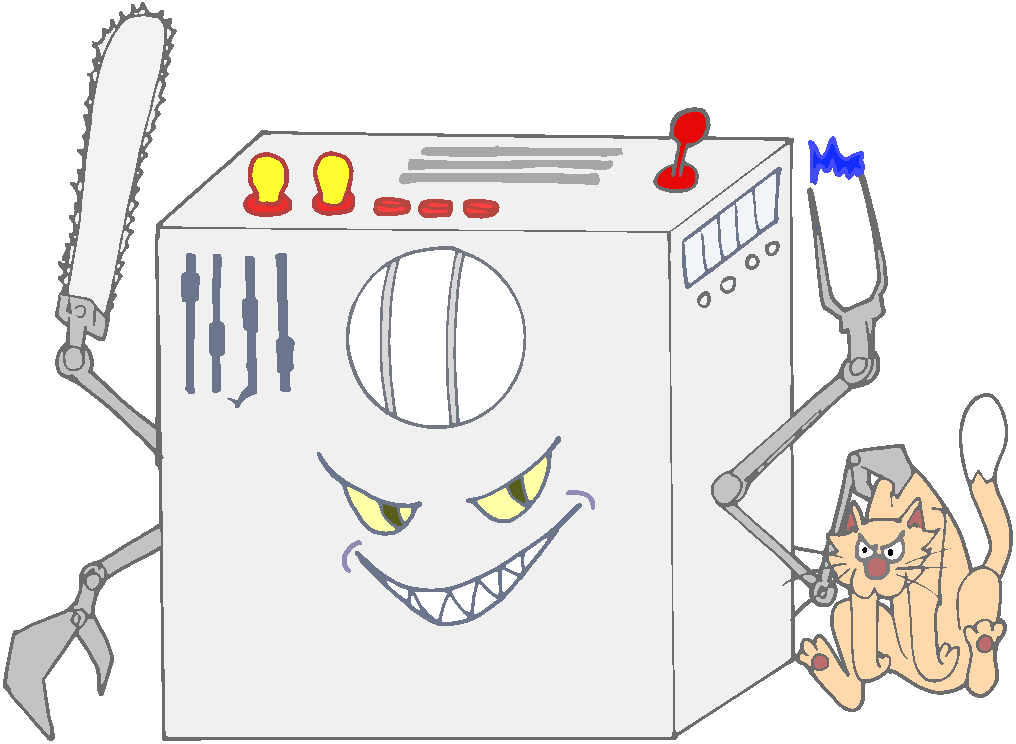
\includegraphics[height=4\textheight]{qc-color}
    };
  \end{tikzpicture}
  \vspace{-2.5cm}
  \usebeamercolor[fg]{titlegraphic}
  {\bf \titlepage}
}

%% 

\begin{frame}{Elliptic curves}

  Let \emph{$E \;:\; y^2 = x^3 + ax + b$} be an elliptic curve\dots

  \begin{center}
    \begin{tikzpicture}[domain=-2.4566:4,samples=100]
      \newcount\rotate
      \animate<2-6>
      \animatevalue<2-6>{\rotate}{0}{90}
      \begin{scope}[rotate=-\the\rotate]
        \draw plot (\x,{0.5*sqrt(\x*\x*\x-4*\x+5)});
        \draw plot (\x,{-0.5*sqrt(\x*\x*\x-4*\x+5)});
      \end{scope}
      
      \begin{uncoverenv}<1>
        \begin{scope}[yscale=1/2]
          \draw[thin,gray,-latex] (0,-7) -- (0,7);
          \draw[thin,gray,-latex] (-3,0) -- (4,0);
          
          \draw (-3,1) -- (4,8/3+3);
          \begin{scope}[every node/.style={draw,circle,inner sep=1pt,fill},cm={1,2/3,0,0,(0,3)}]
            \node at (-2.287980,0) {};
            \node at (-0.535051,0) {};
            \node at (3.267475,0) {};
          \end{scope}
          \begin{scope}[every node/.style={yshift=0.3cm},cm={1,2/3,0,0,(0,3)}]
            \node at (-2.287980,0) {$P$};
            \node at (-0.535051,0) {$Q$};
            \node at (3.267475,0) {$R$};
          \end{scope}
          \draw[dashed] (3.267475,3.267475*2/3+3) -- (3.267475,-3.267475*2/3-3) 
          node[draw,circle,inner sep=1pt,fill] {}
          node[xshift=-0.1cm,anchor=east] {$P+Q$};
        \end{scope}
      \end{uncoverenv}
    \end{tikzpicture}
  \end{center}
\end{frame}

%%

\begin{frame}{Elliptic curves}
  \transdissolve
  \centering
  
\includegraphics[height=0.7\textheight]{ec-happy}
\end{frame}

%%

\begin{frame}{The QUANTHOM Menace}
  \centering
  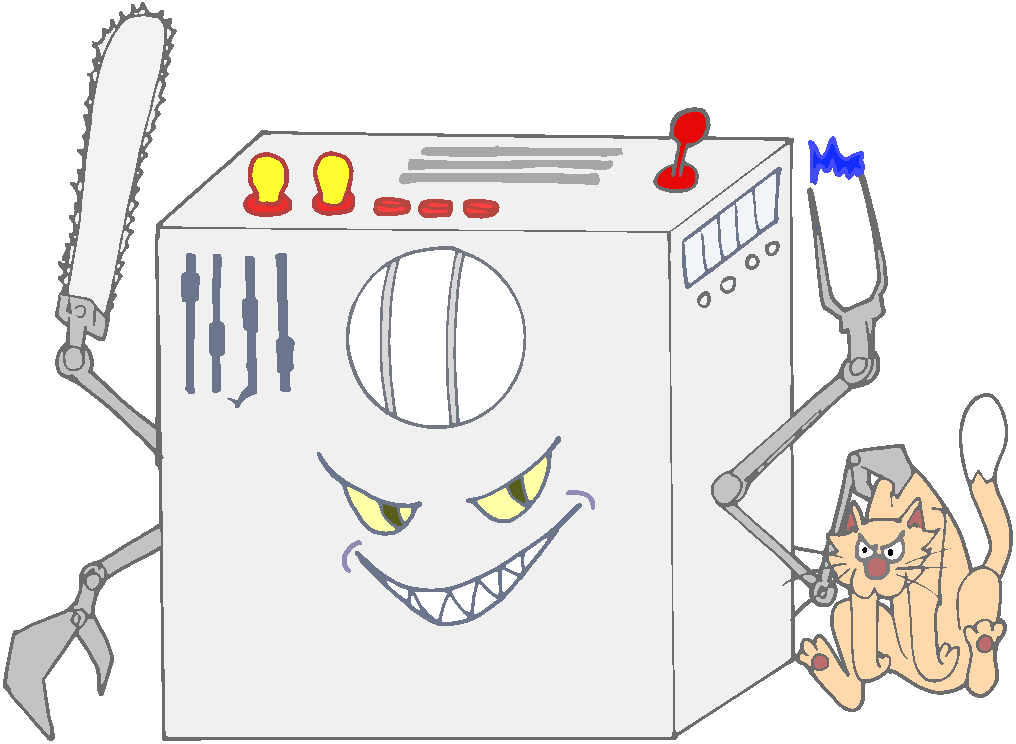
\includegraphics[height=0.7\textheight]{qc-color}
\end{frame}

%%

\begin{frame}{Post-quantum cryptographer?}
  \centering
  \includegraphics[height=0.7\textheight]{ec-broke}
\end{frame}

%%

\begin{frame}{Elliptic curves of the world, UNITE!}
  \centering
  \begin{tikzpicture}
    \foreach \x/\y in {0/-0.5,4/2,8/-1}{
      \node at (\x,\y) {\includegraphics[height=3cm]{ec-banderole}};
    }
    \foreach \x/\y in {1/3,4.5/-1,7/3}{
      \node at (\x,\y) {
\includegraphics[height=3.5cm]{ec-sign}};
    }
    \color{teal!70!blue}\itshape\bfseries\comicneue
    \node[rotate=-3] at (5.9,3.6) {\parbox{0pt}{QUOUSQUE\\QUANTUM?}};
    \node[rotate=-3] at (3.6,-0.4) {\parbox{0pt}{QUANTUM\\SUFFICIT!}};
  \end{tikzpicture}
\end{frame}

%%

\begin{frame}{And so, they found a way around the Quanthom...}
  \centering
  \begin{tikzpicture}
    \comicneue\itshape
    \node at (0,0) {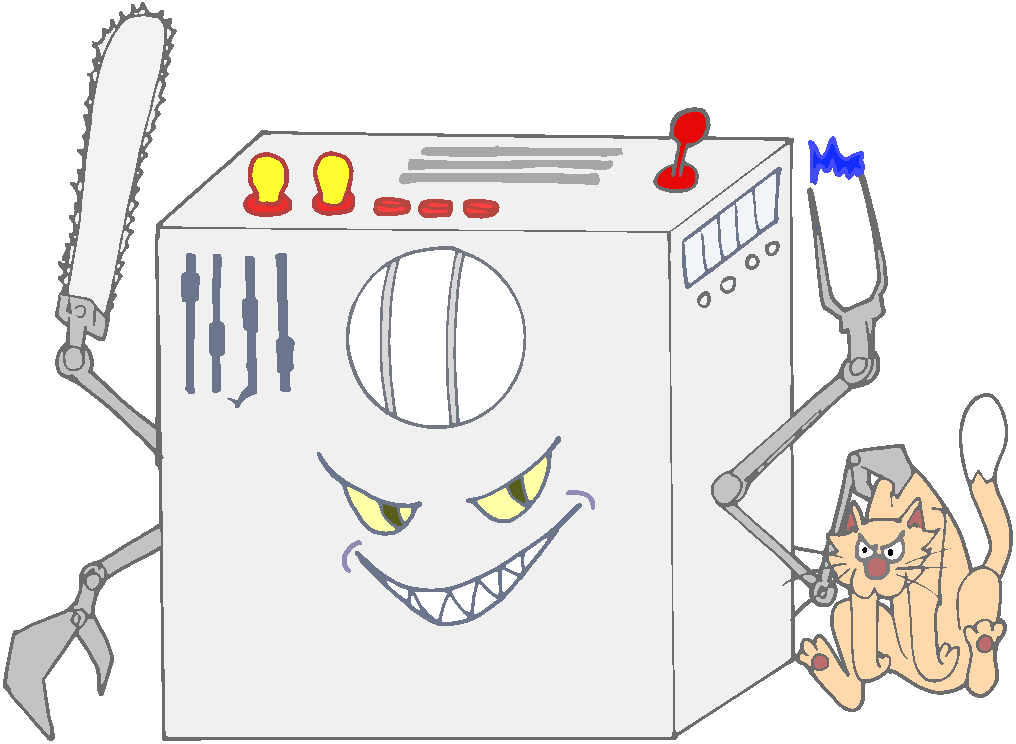
\includegraphics[height=2.5cm]{qc-color}};
    
    \node(E0) at (-5,0) {
\includegraphics[height=1cm]{ec-happy}};

    \uncover<2->{
      \node(EA) at (0,3.5) {
\includegraphics[height=1cm]{ec-happy}};
      \node(EB) at (0,-3.5) {
\includegraphics[height=1cm]{ec-happy}};
      \draw[->,decorate,decoration=snake] (E0) to (EA);
      \draw[->,decorate,decoration=snake] (E0) to (EB);
      \node[right=0.3cm of EA] {\bl{Public curve}};
      \node[right=0.3cm of EB] {\bl{Public curve}};
    }
    \uncover<3>{
      \node(ES) at (5,0) {
\includegraphics[height=1cm]{ec-happy}};
      \draw[->,decorate,decoration=snake] (EA) to (ES);
      \draw[->,decorate,decoration=snake] (EB) to (ES);
      \node[below=1em of ES] {\rd{Shared secret}};
    }
  \end{tikzpicture}
\end{frame}

%%

\begin{frame}{What's an isogeny?}
  \centering
  
\includegraphics[height=2cm]{ec-happy}
  \hfill
  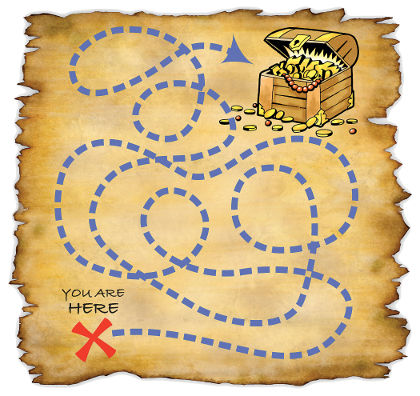
\includegraphics[height=4cm]{map}
  \hfill
  
\includegraphics[height=2cm]{ec-happy}

  \bigskip
  \Large Rebus: 1-3-7-3-8-6
\end{frame}

%%

\begin{frame}
  \frametitle{Isogenies}

  Isogenies are just \alert{the right notion\texttrademark{} of
    morphism} for elliptic curves

  \begin{itemize}
  \item Surjective group morphisms.
  \item Algebraic maps (i.e., defined by polynomials).
  \end{itemize}

  (Separable) isogenies $\Leftrightarrow$ finite subgroups:
  \alert{\[0 \to H \to E \overset{\phi}{\to} E' \to 0\]}
  The kernel \emph{$H$} determines the image curve \emph{$E'$} up to
  isomorphism \[\emph{E/H\overset{\text{\tiny def}}{=}E'}.\]

  \begin{block}{Isogeny degree}
    Neither of these definitions is quite correct, but they
    \textit{nearly} are:
    \begin{itemize}
    \item The degree of \emph{$\phi$} is the cardinality of \emph{$\ker\phi$}.
    \item (\emph{Bisson}) the degree of \emph{$\phi$} is the time
      needed to compute it.
    \end{itemize}
  \end{block}
\end{frame}

%%

\begin{frame}{Isogenies: an example over $\F_{11}$}
  \begin{tikzpicture}[scale=0.4]
    \begin{scope}
      \node[anchor=center] at (0,7) {$E \;:\; y^2 = x^3 + x$};

      \uncover<-1>{
        \draw[thin,gray] (0,-6) -- (0,6);
        \draw[thin,gray] (-6,0) -- (6,0);
      }

      \foreach \x/\y in {0/0,5/3,-4/3,-3/5,-2/1,-1/3} {
        \draw[blue,fill] (\x,\y) circle (0.2) node(E_\x_\y){}
        (\x,-\y) circle (0.2) node(E_\x_-\y){};
      }

      \uncover<4->{\draw[red,fill] (0,0) circle (0.3);}
    \end{scope}

    \draw[black!10!white,thick] (8,-7) -- +(0,14);
    
    \begin{scope}[shift={(16,0)}]
      \node at (0,7) {$E' \;:\; y^2 = x^3 - 4x$};

      \uncover<-1>{
        \draw[thin,gray] (0,-6) -- (0,6);
        \draw[thin,gray] (-6,0) -- (6,0);
      }

      \foreach \x/\y in {0/0,2/0,3/2,4/2,6/4,-2/0,-1/5} {
        \draw[color=blue,fill] (\x,\y) circle (0.2) node(F_\x_\y){}
        (\x,-\y) circle (0.2) node(F_\x_-\y){};
      }
    \end{scope}

    \begin{scope}[color=red,-latex,dashed]
      \begin{uncoverenv}<2->
        \path
        (E_5_3) edge (F_3_2)
        (E_-4_3) edge (F_4_-2)
        (E_-3_5) edge (F_4_2)
        (E_-2_1) edge (F_3_-2)
        (E_-1_3) edge (F_-2_0);
      \end{uncoverenv}
      \begin{uncoverenv}<2,5->
        \path
        (E_5_-3) edge (F_3_-2)
        (E_-4_-3) edge (F_4_2)
        (E_-3_-5) edge (F_4_-2)
        (E_-2_-1) edge (F_3_2)
        (E_-1_-3) edge (F_-2_0);
      \end{uncoverenv}
    \end{scope}
  \end{tikzpicture}
  
  \begin{columns}
    \begin{column}{0.5\textwidth}
      \[\phi(x,y) = \left(\frac{x^2 + 1}{x},\quad y\frac{x^2-1}{x^2}\right)\]
    \end{column}
    \begin{column}{0.5\textwidth}
      \begin{itemize}
      \item<4-> Kernel generator in \alert{red}.
      \item<5-> This is a degree $2$ map.
      \item<6-> Analogous to $x\mapsto x^2$ in $\F_q^*$.
      \end{itemize}
    \end{column}
  \end{columns}
\end{frame}

%%

\begin{frame}
  \frametitle{Easy and hard problems}
  
  \emph{In practice:} an isogeny $\phi$ is just a pair of rational fractions
  
  \alert{\[\frac{N(x)}{D(x)} = \frac{x^n + \cdots + n_1x +
      n_0}{x^{n-1} + \cdots + d_1x + d_0} \in k(x),\qquad\text{with }
    n=\deg\phi,\]}
  
  and $D(x)$ vanishes on $\ker\phi$.

  \vspace{-1mm}
  
  \begin{block}{Vélu's formulas \hfill$\tildO(n)$}
    \begin{description}
    \item[Input:] A generator of the kernel \emph{$H$} of the isogeny.
    \item[Output:] The curve \emph{$E/H$} and the rational fraction \emph{$N/D$}.
    \end{description}
  \end{block}

  \vspace{-2mm}
  
  \begin{block}{The explicit isogeny problem}
    \begin{description}
    \item[Input:] The curves \emph{$E$} and \emph{$E/H$}, the degree
      \emph{$n$}.
    \item[Output:] The rational fraction \emph{$N/D$}.
    \item[Algorithms\footcite{elkies98,couveignes96}]
      \begin{itemize}
        \item Elkies' algorithm (and variants); \hfill \emph{$\tildO(n)$}
        \item Couveignes' algorithm (and variants). \hfill \emph{$\tildO(n^2)$}
      \end{itemize}
    \end{description}
  \end{block}
\end{frame}

%%

\begin{frame}
  \frametitle{Easy and hard problems}

  \begin{block}{Isogeny evaluation}
    \begin{description}
    \item[Input:] A \textit{description} of the isogeny \emph{$\phi$},
      a point \emph{$P\in E(k)$}.
    \item[Output:] The curve \emph{$E/H$} and \emph{$\phi(P)$}.
    \item[Examples]
      \begin{itemize}
      \item \emph{Input =} rational fraction; \hfill $O(n)$
      \item \emph{Input =}
        \alert<2->{composition of \textit{low degree} isogenies; \hfill $\tildO(\log n)$}
      \end{itemize}
    \end{description}
  \end{block}

  \begin{block}{The isogeny walk problem\hfill$O(??)$}
    \begin{description}
    \item[Input:] Isogenous curves \emph{$E$}, \emph{$E'$}.
    \item[Output:] A \emph{path} of \emph{low degree} isogenies from
      $E$ to $E'$.
    \end{description}
  \end{block}
  
  \begin{uncoverenv}<2->
    \begin{center}
      \large
      \textbf{Exponential separation\dots \uncover<3>{Crypto happens!}}
    \end{center}
  \end{uncoverenv}
\end{frame}

%%

\begin{frame}
  \frametitle{Isogeny graphs}
  
  \vspace{-2mm}

  \begin{columns}
    \begin{column}{0.65\textwidth}
      We look at the graph of elliptic curves with isogenies \emph{up
        to isomorphism}.  We say two \alert{isogenies} $\phi,\phi'$
      are \alert{isomorphic} if:
    \end{column}
    \begin{column}{0.3\textwidth}
      \begin{center}
        \begin{tikzpicture}[node distance=4em]
          \node(E){$E$}; 
          \node(E1)[right of=E]{$E'$};
          \node(E2)[below of=E1]{$E'$};
          \scriptsize
          \path[->] (E) edge node[auto]{$\phi$} (E1);
          \path[->] (E) edge node[auto,swap]{$\phi'$} (E2);
          \path[<->] (E1) edge node[rotate=270] {\large$\widetilde{}$} (E2);
        \end{tikzpicture}
      \end{center}
    \end{column}
  \end{columns}

  \emph{Example:} Finite field, ordinary case, graph of isogenies of degree $3$.

  \begin{center}
    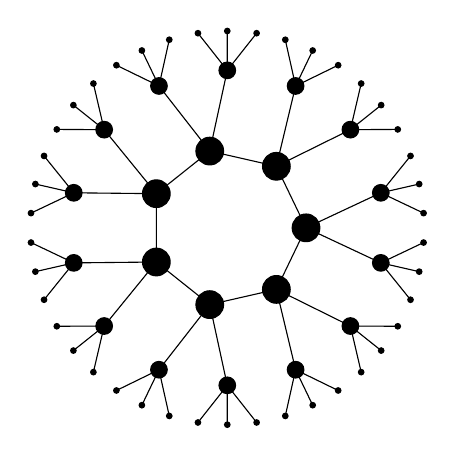
\begin{tikzpicture}[]
      \begin{scope}
        \def\crater{7}
        \foreach \i in {1,...,\crater} {
          \draw[fill] (360/\crater*\i:1cm) circle (5pt);
          \draw (360/\crater*\i : 1cm) -- (360/\crater*\i+360/\crater : 1cm);
          \foreach \j in {-1,1} {
            \draw[fill] (360/\crater*\i : 1cm) -- (360/\crater*\i + \j*360/\crater/4 : 2cm) circle (3pt);
            \foreach \k in {-1,0,1} {
              \draw[fill] (360/\crater*\i + \j*360/\crater/4 : 2cm) --
              (360/\crater*\i + + \j*360/\crater/4 + \k*360/\crater/6 : 2.5cm) circle (1pt);
            }
          }
        }
      \end{scope}
    \end{tikzpicture}
  \end{center}
\end{frame}

%%

\begin{frame}
  \frametitle{Structure of the graph\footcite{deuring41,kohel,fouquet+morain02}}

  \begin{theorem}[Serre-Tate]
    Two curves are isogenous over a finite field $k$ if and only if
    they have the \alert{same number of points} on $k$.
  \end{theorem}

  \begin{block}{The graph of isogenies of \alert{prime} degree \alert{$\ell\ne p$}}
    \emph{Ordinary case (isogeny volcanoes)}
    \begin{itemize}
    \item Nodes can have degree \emph{$0,1,2$} or \emph{$\ell+1$}.
      \begin{itemize}
      \item  For $\sim 50\%$ of the primes $\ell$, graphs are just isolated
        points;
      \item For other $\sim 50\%$, graphs are $2$-regular;
      \item other cases only happen for finitely many $\ell$'s.
      \end{itemize}
    \end{itemize}
    
    \emph{Supersingular case (algebraic closure)}
    \begin{itemize}
    \item The graph is \emph{$\ell+1$-regular}.
    \item There is a \alert{unique (finite) connected component} made
      of all supersingular curves with the same number of points.
    \end{itemize}
  \end{block}
\end{frame}

%%

\begin{frame}{Expander graphs from isogenies}
  \begin{block}{Expander graphs}
    An infinite family of connected $k$-regular graphs on $n$ vertices
    is an \emph{expander family} if there exists an $\epsilon>0$ such
    that all \emph{non-trivial} eigenvalues satisfy
    $|\lambda| \le (1-\epsilon)k$ for $n$ large enough.
    \begin{itemize}
    \item Expander graphs have \emph{short diameter} ($O(\log n)$);
    \item Random walks \emph{mix rapidly} (after $O(\log n)$ steps,
      the induced distribution on the vertices is close to uniform).
    \end{itemize}
  \end{block}

  \begin{description}
  \item[Supersingular] Let $\ell$ be fixed, the graphs of all supersingular curves
    with $\ell$-isogenies are expanders;\footcite{pizer1,pizer2}
  \item[Ordinary*] Let $\O\subset\Q[\sqrt{-D}]$ be an order in a
    quadratic imaginary field. The graphs of all curves over $\F_q$
    with \emph{complex multiplication by $\O$}, with isogenies of
    prime degree bounded by $(\log q)^{2+\delta}$, are
    expanders.\footcite{jao+miller+venkatesan09} \hfill{\tiny *(may contain traces of GRH)}
  \end{description}
\end{frame}

%%

\begin{frame}
  \frametitle{The first 10 years of isogeny based cryptography}

  \begin{description}
  \item<1->[1996] Couveignes suggests \emph{isogeny-based
      key-exchange} at a seminar in École Normale Supérieure;
  \item<1->[1997] He submits \emph{``Hard Homogeneous Spaces''} to
    Crypto;
  \item<2->[1997] His paper gets \alert{rejected};
  \item<3->[1997--2006] \dots Nothing happens for about 10 years.
  \end{description}

  \bigskip
  
  \begin{uncoverenv}<4->
    \begin{center}
      \large
      
      \emph{Ok. Let's move on to the next 10 years!}
    \end{center}
  \end{uncoverenv}
\end{frame}

%%

\begin{frame}
  \frametitle{Isogeny walks and
    cryptanalysis\footcite{galbraith99,GHS,bisson+sutherland11-rho}}
  
  \emph{Fact:} Having a \emph{weak DLP} is not (always) isogeny invariant.

  \begin{center}
    \begin{tikzpicture}
      \path (0,0) node[anchor=east] {$E$} (6,0) node[anchor=west] {$E'$};
      \path[gray] (-0.8,0) node[anchor=east] {weak curve}
      (6.8,0) node[anchor=west] {strong curve};

      \draw[->] (0,0) -- (0.5,-0.2);
      \draw[->] (6,0) -- (5.5,0.2);
      \draw[->] (0.5,-0.2) -- (1,0.2);
      \draw[->] (5.5,0.2) -- (5,-0.2);
      \begin{scope}[densely dotted,coils/.style={decorate,decoration={coil,aspect=0,amplitude=2pt}}]
        \draw[coils] (1,0.2) -- (3,0.4);
        \draw[coils] (5,-0.2) -- (3,0.4);
        \draw[-angle 90,coils] (3,0.4) -- (3, -0.4) node[anchor=north] {$E''$};
      \end{scope}
    \end{tikzpicture}
  \end{center}
  
  \begin{block}{Fourth root attacks}
    \begin{itemize}
    \item Start two random walks from the two curves and wait for a
      collision.
    \item Over \emph{$\F_q$}, the average size of an isogeny class is
      \emph{$h_\Delta\sim\sqrt{q}$}.
    \item A collision is expected after \emph{$O(\sqrt{h_\Delta}) =
        O(q^{\frac{1}{4}})$} steps.
    \end{itemize}
  \end{block}

  \emph{Note:} Can be used to build \emph{trapdoor
    systems}\footcite{teske06}.

\end{frame}

%% 

\begin{frame}
  \frametitle{Random walks and hash functions}

  Any expander graph gives rise to a hash function.

  \begin{center}
    \begin{tikzpicture}
      \coordinate (last) at (0,0);
      \draw (last) node[anchor=east] {$v$};
      \foreach \i in {1,...,6} {
        \pgfmathparse{(-1)^\i}
        \let\sign\pgfmathresult
        \pgfmathparse{int(mod(\i+1,2))}
        \let\bit\pgfmathresult
        \pgfmathparse{int(mod(\i,2))}
        \let\nbit\pgfmathresult
        \draw[->] (last) -- (\i,\sign*0.1) node[blue,pos=0.5,yshift=\sign*0.2cm]{\small$\bit$};
        \draw[dashed,->] (last) -- (\i,-\sign*0.5) node[gray,pos=0.5,yshift=-\sign*0.2cm]{\small$\nbit$};
        \coordinate (last) at (\i,\sign*0.1);
      }
      \draw (last) node[anchor=west] {$v'$};

      \node[blue,anchor=west] at (7,0) {$H(010101)=v'$};
    \end{tikzpicture}
  \end{center}

  \begin{itemize}
  \item Fix a starting vertex \emph{$v$};
  \item The value to be hashed determines a random path to \emph{$v'$};
  \item \emph{$v'$} is the hash.
  \end{itemize}

  \begin{block}{Provably secure hash functions}
    \begin{itemize}
    \item Use the expander graph of \alert{supersingular
        $2$-isogenies};\footcite{charles+lauter+goren09}
    \item \alert{Collision resistance} = hardness of finding cycles in the graph;
    \item \alert{Preimage resistance} = hardness of finding a path
      from \emph{$v$} to \emph{$v'$}.
    \end{itemize}
  \end{block}
\end{frame}

%%

\begin{frame}
  \frametitle{Random walks and key exchange}

  \begin{flushleft}
    \Large
    Let's try something harder...
  \end{flushleft}

  \begin{center}
    \begin{tikzpicture}[xscale=0.7,yscale=0.4]
      \foreach \p/\psym/\psign in {Alice/A/-1,Bob/B/1} {
        \coordinate (last) at (\psign,0);
        \foreach \round in {0,1} {
          \pgfmathparse{\psign*(2*\round-1)}
          \let\rsign\pgfmathresult
          \foreach \i in {1,...,5} {
            \pgfmathparse{int(mod(mod(\i,2+(1+\psign)*0.5+\round),2))}
            \let\bit\pgfmathresult
            \pgfmathparse{int(mod(\bit+1,2))}
            \let\nbit\pgfmathresult
            \pgfmathparse{(-1)^(\bit)}
            \let\sign\pgfmathresult
            \draw[->] (last) -- ++(-\rsign,-1+\sign*0.1) node[blue,pos=0.5,yshift=\sign*0.1cm,xshift=-\sign*0.1cm*\rsign]{\small$\bit$};
            \draw[dashed,->,white!80!black] (last) -- ++(-\rsign+\sign*0.5*\rsign,-1-\sign*0.5) node[pos=0.5,yshift=-\sign*0.1cm,xshift=\sign*0.1cm*\rsign]{\small$\nbit$};
            \coordinate (last) at (-\i*\rsign+\round*5*\rsign+\psign,-\i-\round*6.6+\sign*0.1);
          }
          \coordinate (last) at (-5*\rsign+\psign,-6.6);
        }
      }
      \draw[alert] (0,0) node[anchor=south] {Public $v_0$}
      (-5,-5.2) node[anchor=north] {Alice's public $v_A$}
      (5,-5.2) node[anchor=north] {Bob's public $v_B$}
      (0,-11.8) node[anchor=north] {Shared secret};
    \end{tikzpicture}
  \end{center}

  \vspace{-1cm}
  
  \begin{flushright}
    \Large
    ...is this even possible?
  \end{flushright}
\end{frame}

%%

\begin{frame}
  \frametitle{Expander graphs from groups}
  \begin{center}
    \begin{tikzpicture}
      \begin{scope}
        \def\crater{12}
        \def\jumpa{-8}
        \def\jumpb{9}
        \def\diam{3cm}

        \foreach \i in {1,...,\crater} {
          \uncover<2->{\draw[blue] (360/\crater*\i : \diam) to[bend right] (360/\crater*\i+360/\crater : \diam);}
          \uncover<3->{\draw[red] (360/\crater*\i : \diam) to[bend right] (360/\crater*\i+\jumpa*360/\crater : \diam);}
          \uncover<4->{\draw[green] (360/\crater*\i : \diam) to[bend right=50] (360/\crater*\i+\jumpb*360/\crater : \diam);}
        }
        \foreach \i in {1,...,\crater} {
          \pgfmathparse{int(mod(2^\i,13))}
          \let\exp\pgfmathresult
          \draw[fill] (360/\crater*\i: \diam) circle (2pt) +(360/\crater*\i: 0.4) node{$g^{\exp}$};
        }
      \end{scope}
      \begin{scope}[xshift=4cm]
        \draw (0,2.1) node[anchor=west] {\parbox{4cm}{
            Let \emph{$G=\langle g\rangle$} be a cyclic group of order \emph{$p$}.
            \uncover<2->{Let \emph{$S\subset(\Z/p\Z)^\times$} s.t. \emph{$S^{-1}\subset S$}.\\
              The \emph{Schreier graph} of \emph{$(S,G\setminus\{1\})$} is (usually) an expander.}}};
        \uncover<2->{\draw[blue] (0,0) -- (0.5,0) (0.5,0) node[anchor=west] {$x \mapsto x^{2}$};}
        \uncover<3->{\draw[red] (0,-1) -- (0.5,-1) (0.5,-1) node[anchor=west] {$x \mapsto x^{3}$};}
        \uncover<4->{\draw[green] (0,-2) -- (0.5,-2) (0.5,-2) node[anchor=west] {$x \mapsto x^{5}$};}
      \end{scope}
    \end{tikzpicture}
  \end{center}
\end{frame}

%% 

{
  \newcommand{\myedge}[3]{
    \draw[#3] (360/\crater*#1 : \diam) to[bend right] (360/\crater*#2 : \diam);
  }

\begin{frame}
  \frametitle{Key exchange from Schreier graphs}

  \begin{columns}
    \begin{column}{0.55\textwidth}
      \begin{tikzpicture}
        \begin{scope}
          \def\crater{12}
          \def\jumpa{-8}
          \def\jumpb{9}
          \def\diam{2.5cm}
          
          \foreach \i in {1,...,\crater} {
            \pgfmathparse{int(mod(2^\i,13))}
            \let\exp\pgfmathresult
            \draw[fill] (360/\crater*\i: \diam) circle (2pt);
          }
          \uncover<2,6->{
            % Alice 1
            \myedge{0}{1}{blue}\myedge{1}{5}{red}\myedge{5}{6}{blue}\myedge{6}{3}{green}
          }
          \uncover<3,5>{
            % Bob 1
            \begin{scope}[dashed,thick]
              \myedge{0}{4}{red}\myedge{4}{8}{red}\myedge{8}{5}{green}\myedge{5}{6}{blue}
            \end{scope}
          }
          \uncover<5>{
            % Alice 2
            \myedge{6}{7}{blue}\myedge{7}{11}{red}\myedge{11}{0}{blue}\myedge{0}{9}{green}
          }
          \uncover<6->{
            % Bob 2
            \begin{scope}[dashed,thick]
              \myedge{3}{7}{red}\myedge{7}{11}{red}\myedge{11}{8}{green}\myedge{8}{9}{blue}
            \end{scope}
          }

          \draw (0 : \diam + 0.4cm) node {$g$};
          \uncover<2->{\draw (360/\crater*3 : \diam + 0.4cm) node {$g_A$};}
          \uncover<3->{\draw (360/\crater*6 : \diam + 0.4cm) node {$g_B$};}
          \uncover<5->{\draw (360/\crater*9 : \diam + 0.4cm) node {$g_{BA}\uncover<6->{=g_{AB}}$};}
        \end{scope}
      \end{tikzpicture}  
    \end{column}    
    \begin{column}{0.45\textwidth}
      \begin{onlyenv}<-6>
        \textbf{Public parameters:}
        \begin{itemize}
        \item A group \emph{$G=\langle g\rangle$} of order \emph{$p$};
        \item A subset \emph{$S\subset(\Z/p\Z)^\times$}.
        \end{itemize}
        \begin{enumerate}
        \item<2-> \textbf{Alice} takes a \alert{secret} random walk
          \emph{$s_A:g\to g_A$} of length \emph{$O(\log p)$};
        \item<3-> \textbf{Bob} does the same;
        \item<4-> They publish \emph{$g_A$} and \emph{$g_B$};
        \item<5-> \textbf{Alice} repeats her secret walk \emph{$s_A$}
          starting from \emph{$g_B$}.
        \item<6-> \textbf{Bob} repeats his secret walk \emph{$s_B$}
          starting from \emph{$g_A$}.
        \end{enumerate}
      \end{onlyenv}
      \begin{onlyenv}<7->
        \textbf{Why does this work?}
        \begin{align*}
          g_A &= g^{\bl{2}\cdot\rd{3}\cdot\bl{2}\cdot\gr{5}},\\
          g_B &= g^{\rd{3^2}\cdot\gr{5}\cdot\bl{2}},\\
          g_{BA} &= g_{AB} = g^{\bl{2^3}\cdot\rd{3^3}\cdot\gr{5^2}};
        \end{align*}
        and $g_A,g_B,g_{AB}$ are (nearly) uniformly distributed in $G$\dots

        \bigskip
        
        \begin{uncoverenv}<8->
          \dots Indeed, this is just a twisted presentation of the
          \alert{classical Diffie-Hellman protocol!}
        \end{uncoverenv}
      \end{onlyenv}
    \end{column}
  \end{columns}
\end{frame}
}

%%

\begin{frame}
  \frametitle{Group action on isogeny graphs}

  \begin{columns}
    \begin{column}{0.5\textwidth}
      \centering
      \begin{tikzpicture}
        \begin{scope}
          \def\crater{11}
          \def\jump{5}
          \def\diam{2.5cm}

          \foreach \i in {1,...,\crater} {
            \draw[blue] (360/\crater*\i : \diam) to[bend right] (360/\crater*\i+360/\crater : \diam);
            \draw[red] (360/\crater*\i : \diam) to[bend left] (360/\crater*\i+\jump*360/\crater : \diam);
          }
          \foreach \i in {1,...,\crater}
          \draw[fill] (360/\crater*\i: \diam) circle (2pt);
        \end{scope}
        \begin{scope}[xshift=-1.5cm, yshift=-3.2cm]
          \draw[blue] (0,0) -- (0.5,0) (0.5,0) node[anchor=west] {\bl{$\ell_1$}-isogenies};
          \draw[red] (0,-1) -- (0.5,-1) (0.5,-1) node[anchor=west] {\rd{$\ell_2$}-isogenies};
        \end{scope}
      \end{tikzpicture}
    \end{column}
    \begin{column}{0.5\textwidth}
      \begin{itemize}
      \item There is a group action of the \emph{ideal class group}
        $\Cl(\O)$ on the set of ordinary curves with \emph{complex
          multiplication} by $\O$.
      \item Its Schreier graph is an isogeny graph (and an
        expander if we take enough generators)
      \end{itemize}
    \end{column}
  \end{columns}
\end{frame}

%%

\begin{frame}[plain]
  \centering
  \begin{tikzpicture}
    \node at (0,0) {\includegraphics[height=0.77\textwidth]{ec-banderole}};
    \draw[decorate,decoration={
        text along path,text align=center,
        text={|\Huge\comicneue\bfseries\color{teal!70!blue}|Class Group Action}
      }] (-5,2.5) to[bend right=25] (5,2.5);
  \end{tikzpicture}
\end{frame}

%%

\begin{frame}
  \frametitle{Key exchange in graphs of ordinary isogenies\footcite{Couv,R&S} (CRS)}
  
  \emph{Parameters:}
  \begin{itemize}
  \item \emph{$E/\F_p$ ordinary elliptic curve},
  \item (small) primes \bl{$\ell_1$},\rd{$\ell_2$},\dots
    such that $\left(\frac{D_\pi}{\ell_i}\right)=1$.
  \item elements
    \bl{$\frak f_1=(\ell_1,\pi-\lambda_1)$},\rd{$\frak f_2=(\ell_2,\pi-\lambda_2)$} in
    $\Cl(\O)$.
  \end{itemize}

  \emph{Secret data:} \emph{Random walks} $\a,\b\in\Cl(\O)$ in the
  isogeny graph.
  
  \begin{center}
    \begin{tikzpicture}
      \Large
      \node[matrix of math nodes, ampersand replacement=\&, column sep=0cm, row sep=1cm] (diagram) {
        \& |(1)| E \\
        |(a)| \a\ast E \& \& |(b)| \b\ast E\\
        \& |(ab)| \a\b\ast E = \b\a\ast E\\
      };
      \small
      \path[->] (1) edge node[auto,swap]{$\bl{(\frak f_1)^{a_1}}\rd{(\frak f_2)^{a_2}}\cdots=\a$} (a);
      \path[->] (1) edge node[auto]{$\b=\bl{(\frak f_1)^{b_1}}\rd{(\frak f_2)^{b_2}}\cdots$} (b);
      \path[->] (a) edge (ab);
      \path[->] (b) edge (ab);
    \end{tikzpicture}
  \end{center}
\end{frame}

%%

\begin{frame}
  \frametitle{CRS key exchange}

  \begin{center}
    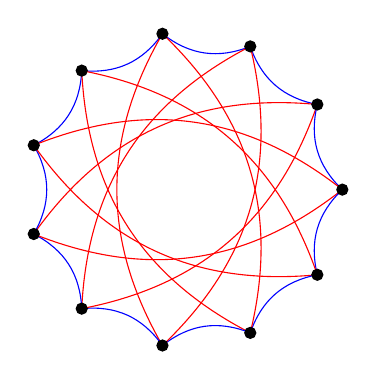
\begin{tikzpicture}
      \begin{scope}
        \def\crater{11}
        \def\jump{5}
        \def\diam{2cm}

        \foreach \i in {1,...,\crater} {
          \draw[blue] (360/\crater*\i : \diam) to[bend left] (360/\crater*\i+360/\crater : \diam);
          \draw[red] (360/\crater*\i : \diam) to[bend right] (360/\crater*\i+\jump*360/\crater : \diam);
        }
        \foreach \i in {1,...,\crater}
          \draw[fill] (360/\crater*\i: \diam) circle (2pt);
      \end{scope}
    \end{tikzpicture}
  \end{center}

  \begin{description}
  \item[Key generation:] compose small degree
    isogenies\\\alert{polynomial in the lenght of the random walk}.
  \item[Attack:] find an isogeny between two curves\\\alert{polynomial
      in the degree, exponential in the length}.
  \item[In practice\footcite{defeo-kieffer-smith}:] 5 minutes for a
    key exchange at 128-bits security level\dots
  \end{description}
\end{frame}

%%

\begin{frame}{CSIDH \textit{(pron.: Seaside)}\footcite{csidh}}
  \begin{block}{One walk step in CRS: the \emph{explicit isogeny problem}}
    \begin{description}
    \item[Input:] Curves \emph{$E$} and \emph{$E/H$}, an isogeny degree
      \emph{$\ell_i$}.
    \item[Output:] The rational fraction \emph{$N/D$}.
    \item[Algorithm:] Elkies' algorithm (very expensive). \hfill
      \emph{$\tildO(n)$}
    \end{description}
  \end{block}

  \begin{block}{CSIDH: Key observations}
    \begin{enumerate}
    \item If we know the kernel \emph{$H$} in advance, we can apply
      \emph{Vélu's formulas} (much faster than Elkies).
    \item If the curves are \emph{supersingular}, it is very easy to
      control the kernels.
    \item If we restrict to supersingular isogenies \emph{defined over
        $\F_p$}, the isogeny graph structure is \emph{identical} to
      CRS!\footcite{DelfsG16}
    \end{enumerate}
  \end{block}

  \centering
  \textbf{Result:} Same security as CRS in less than 100ms!
\end{frame}

%%

\begin{frame}{CRS and CSIDH: quantum security}

  \textbf{Fact:} Shor's algorithm \emph{does not apply} to Diffie-Hellman
  protocols from \emph{group actions}.

  \begin{block}{Subexponential attack\hfill\emph{$\exp(\sqrt{\log p\log\log p})$}}
    \begin{itemize}
    \item Reduction to the \emph{hidden shift problem} by evaluating
      the class group action in \emph{quantum
        supersposition}~\footcite{childs+jao+soukharev10} (subexpoential cost);
    \item Well known reduction from the hidden shift to the
      \emph{dihedral (non-abelian) hidden subgroup problem};
    \item Kuperberg's algorithm\footcite{Kup,regev04,Kuperberg2013}
      solves the dHSP with a subexponential number of class group
      evaluations.
    \end{itemize}
  \end{block}
\end{frame}

%%

\begin{frame}
  \frametitle{Key exchange in the full supersingular graph}
  
  \begin{description}
  \item[Good news:] there is no action of a commutative class group.
  \item[Bad news:] there is no action of a commutative class group.
  \end{description}

  \alert{However:} an algebraic structure is still acting on
  supersingular graphs: \emph{ideals of maximal orders of a quaternion
    algebra}.

  \begin{center}
    \begin{tikzpicture}
      \large
      \node[matrix of nodes, ampersand replacement=\&, column sep=3cm, row sep=1.5cm] (diagram) {
        |(E)| $E$ \& |(Es)| $E'$ \\
        |(Ep)| {$E''$} \& |(Eps)| {$E'''$}\\
      };
      \path[blue,->] (E) edge node[auto] {$\a$} (Es);
      \path[blue,->] (Ep) edge node[auto,swap] {$\a_\b$} (Eps);
      \path[red,->] (E) edge node[auto,swap] {$\b$} (Ep);
      \path[red,->] (Es) edge node[auto] {$\b_\a$} (Eps);
    \end{tikzpicture}
  \end{center}

  \begin{itemize}
  \item The action is \alert{not commutative}, we cannot use the same
    technique;
  \item We let instead Alice and Bob walk in two \alert{different
      isogeny graphs} on the \alert{same vertex set}.
  \end{itemize}
\end{frame}

%%

\begin{frame}
  \frametitle{Key exchange with supersingular curves}

  In practice, we fix:

  \begin{itemize}
  \item Small primes \bl{$\ell_A$}, \rd{$\ell_B$};
  \item A large prime \emph{$p$} such that $p+1 =
    \bl{\ell_A^{e_A}}\rd{\ell_B^{e_B}}$;
  \item A supersingular curve \emph{$E$} over \emph{$\F_{p^2}$}, such that
    \[E \simeq (\Z/(p+1)\Z)^2 = \bl{(\Z/\ell_A^{e_A}\Z)^2} \oplus \rd{(\Z/\ell_B^{e_B}\Z)^2},\]
  \item We use isogenies of degrees \bl{$\ell_A^{e_A}$} and
    \rd{$\ell_B^{e_B}$} with \emph{cyclic rational kernels};
  \item The diagram below can be constructed in time
    $\text{poly}(\bl{e_A}+\rd{e_B})$.
  \end{itemize}

  \begin{center}
    \begin{tikzpicture}
      \begin{scope}
        \draw (0,1.2) node[anchor=east,blue] {$\ker\phi=\cyc{P}\subset E[\ell_A^{e_A}]$};
        \draw (0,0.4) node[anchor=east,red] {$\ker\psi=\cyc{Q}\subset E[\ell_B^{e_B}]$};
        \draw (0,-0.4) node[anchor=east,blue] {$\ker\phi' = \cyc{\rd{\psi}(P)}$};
        \draw (0,-1.2) node[anchor=east,red] {$\ker\psi' = \cyc{\bl{\phi}(Q)}$};
      \end{scope}
      \begin{scope}[xshift=4.5cm]
        \large
        \node[matrix of nodes, ampersand replacement=\&, column sep=3cm, row sep=1.5cm] (diagram) {
          |(E)| $E$ \& |(Es)| $E/\cyc{\bl{P}}$ \\
          |(Ep)| {$E/\cyc{\rd{Q}}$} \& |(Eps)| {$E/\cyc{\bl{P},\rd{Q}}$}\\
        };
        \path[->,blue] (E) edge node[auto] {$\phi$} (Es);
        \path[->,blue] (Ep) edge node[auto,swap] {$\phi'$} (Eps);
        \path[->,red] (E) edge node[auto,swap] {$\psi$} (Ep);
        \path[->,red] (Es) edge node[auto] {$\psi'$} (Eps);
      \end{scope}
    \end{tikzpicture}
  \end{center}
\end{frame}

%%

\begin{frame}
  \frametitle{Supersingular Isogeny
    Diffie-Hellman\footcite{jao+defeo2011,defeo+jao+plut12}}

  \vspace{-1cm}

  \begin{columns}
    \begin{column}{0.4\textwidth}
      \begin{block}{}
        \emph{Parameters:}
        \begin{itemize}
          \setlength{\itemsep}{1.5ex}
        \item Prime $p$ such that $p+1 = \bl{\ell_A^a}\rd{\ell_B^b}$;
        \item Supersingular curve \emph{$E\simeq (\Z/(p+1)\Z)^2$};
        \item \bl{$E[\ell_A^a] = \cyc{P_A,Q_A}$};
        \item \rd{$E[\ell_B^b] = \cyc{P_B,Q_B}$}.
        \end{itemize}

        \emph{Secret data:}
        \begin{itemize}
          \setlength{\itemsep}{1.5ex}
        \item \bl{$R_A = m_AP_A + n_AQ_A$},
        \item \rd{$R_B = m_BP_B + n_BQ_B$},
        \end{itemize}
      \end{block}
    \end{column}
    \begin{column}{0.58\textwidth}
      \begin{center}
        \begin{tikzpicture}
          \large
          \node[matrix of nodes, ampersand replacement=\&, column sep=4mm, row sep=2cm] (diagram) {
            \& |(1)| $E$ \\
            |(a)| \parbox{1.5cm}{$E/\cyc{\bl{R_A}}$\\\uncover<2->{{\footnotesize $\bl{\phi(}\rd{P_B}\bl{)}\\\bl{\phi(}\rd{Q_B}\bl{)}$}}} \& \&
            |(b)| \parbox{1.5cm}{$E/\cyc{\rd{R_B}}$\\\uncover<2->{{\footnotesize $\rd{\psi(}\bl{P_A}\rd{)}\\\rd{\psi(}\bl{Q_A}\rd{)}$}}}\\
            \normalsize $\frac{E/\cyc{\bl{R_A}}}{\alert{\bl{\phi(}\rd{R_B}\bl{)}}} \simeq$ \&
            |(ab)|  $E/\cyc{\bl{R_A},\rd{R_B}}$ \&
            \normalsize $\simeq \frac{E/\cyc{\rd{R_B}}}{\alert{\rd{\psi(}\bl{R_A}\rd{)}}}$\\
          };
          \small
          \path[blue] (1) edge node[auto,swap](phia) {$\phi$} (a);
          \path[red] (1) edge node[auto](phib) {$\psi$} (b);
          \path[red] (a) edge node[auto,swap](psia){$\psi'$} (ab);
          \path[blue] (b) edge node[auto](psib){$\phi'$} (ab);
          \uncover<3>{\path[dashed,->] (phia) edge node[auto]{\footnotesize $\bl{\phi(}\rd{R_B}\bl{)}$} (psia);}
          \uncover<3>{\path[dashed,->] (phib) edge node[auto,swap]{\footnotesize $\rd{\psi(}\bl{R_A}\rd{)}$} (psib);}
        \end{tikzpicture}
      \end{center}  
    \end{column}
  \end{columns}
\end{frame}

%%

\begin{frame}{CSIDH vs SIDH}
  \centering
  \begin{tabular}{l | c | c}
    & \textbf{CSIDH} & \textbf{SIDH}\\
    \hline
    Speed @128b & <100ms & 10ms\\
    Public key size @128b & 64B & 378B\\
    Submitted to NIST & no & yes\\
    Best classical attack & $p^{1/4}$ & $p^{1/4}$\\
    Best quantum attack & subexponential & $p^{1/6}$\\
    Key size scales & quadratically & linearly\\
    Security assumption & isogeny walk problem & ad hoc\\
    CPA security & yes & yes\\
    CCA security & yes & Fujsaki-Okamoto\\
    Non-interactive key ex. & yes & no\\
    Signatures & unclear & very slow
  \end{tabular}
  
\end{frame}

%%

\begin{frame}{SIKE: Supersingular Isogeny Key Encapsulation}
  \begin{itemize}
  \item Submission to the \emph{NIST PQ competition}:
    \begin{description}
    \item[SIKE.PKE:] El Gamal-type system with \emph{IND-CPA} security
      proof,
    \item[SIKE.KEM:] generically transformed system with
      \emph{IND-CCA} security proof.
    \end{description}
  \item Security levels 1, 3 and 5.
  \item \emph{Smallest communication complexity} among all proposals
    in each level.
  \item \emph{Slowest} among all benchmarked proposals in each level.
  \item A team of 14 submitters, from 8 universities and companies.
  \item Visit \url{https://sike.org/}.
  \end{itemize}

  \centering
  \begin{tabular}{l | c c c c c }
    & $p$ & cl. security & q. security & speed & comm.\\
    \hline
    SIKEp503 & $2^{250}3^{159}-1$ & 126 bits & 84 bits & 10ms & 0.4KB\\
    SIKEp751 & $2^{372}3^{239}-1$ & 188 bits & 125 bits & 30ms & 0.6KB\\
    SIKEp964 & $2^{486}3^{301}-1$ & 241 bits & 161 bits & & 0.8KB
  \end{tabular}
\end{frame}

%%

\begin{frame}
  \centering
  \begin{tikzpicture}
    \begin{scope}[xscale=1.2,black!60]
      \def\crater{7}
      \foreach \i in {1,...,\crater} {
        \draw[fill] (360/\crater*\i:3cm) circle (5pt);
        \draw (360/\crater*\i : 3cm) -- (360/\crater*\i+360/\crater : 3cm);
        \foreach \j in {-1,1} {
          \draw[fill] (360/\crater*\i : 3cm) -- (360/\crater*\i + \j*360/\crater/4 : 4cm) circle (3pt);
          \foreach \k in {-1,0,1} {
            \draw[fill] (360/\crater*\i + \j*360/\crater/4 : 4cm) --
            (360/\crater*\i + + \j*360/\crater/4 + \k*360/\crater/6 : 4.5cm) circle (1pt);
          }
        }
      }
    \end{scope}
    
    \draw (0,1) node{\Huge\bf Thank you};
    \draw (0,-0.6) node{\large\url{https://defeo.lu/}};
    \draw (0,-1.3) node{\large
\includegraphics[height=0.9em]{twitter.png}~\href{https://twitter.com/luca_defeo}{@luca\_defeo}};
  \end{tikzpicture}
\end{frame}

%%
%%

\begin{frame}[allowframebreaks]
  \frametitle{References}

  \defbibfilter{books}{\type{book} \or \type{booklet} \or \type{thesis}
    \or \type{report} \or \type{collection} \or \type{manual}
    \or \type{periodical} \or \type{proceedings}}
  \defbibfilter{articles}{\not \(\type{book} \or \type{booklet} \or \type{thesis}
    \or \type{report} \or \type{collection} \or \type{manual}
    \or \type{periodical} \or \type{proceedings}\)}

  \beamertemplatebookbibitems
  \printbibliography[filter=books]
  \beamertemplatearticlebibitems
  \printbibliography[filter=articles]
\end{frame}

\end{document}


% LocalWords:  Isogeny abelian isogenies hyperelliptic supersingular Frobenius
% LocalWords:  isogenous


